\documentclass[a4paper, 10pt]{article}
\usepackage{fullpage} % changes the margin
\usepackage[english]{babel}
\usepackage[utf8]{inputenc}
\usepackage{hyperref}
\usepackage{xcolor}
\usepackage{graphicx}
\usepackage{array}
\usepackage{float}
\usepackage{longtable}
\usepackage[bottom]{footmisc}
\usepackage{cite}
\usepackage{parskip}
\usepackage{subcaption}
\usepackage{amssymb}
\usepackage{amsmath}
\usepackage{listings}
\usepackage[nocenter]{qtree}
\usepackage{tree-dvips}
\usepackage{multirow}

\hypersetup{
	colorlinks=true,       % false: boxed links; true: colored links
	linkcolor=blue,        % color of internal links
	citecolor=blue,        % color of links to bibliography
	filecolor=magenta,     % color of file links
	urlcolor=blue
}

%\setlength{\parindent}{0cm}
\newcommand{\code}[1]{\texttt{#1}}
\newcommand{\suchthat}[0]{\hspace{1mm}|\hspace{1mm}}
\renewcommand{\arraystretch}{1.4}
\definecolor{statement}{gray}{0.5}

\graphicspath{{img/}}

\begin{document}

\noindent
\begin{flushright}
    \large\textbf{Miguel Alcón Doganoc} \\
    Algorithms for VLSI \\
    \today
\end{flushright}

\noindent
{\huge{\textbf{Exercises on logic synthesis}}}

\section{Two-level minimization}
{\color{statement} 
Let us consider the following incompletely specified function, where $f$ represents the on-set and d the don’t care set:
\begin{align*}
    f &= \bar{a}\bar{b}c + bc\bar{d} + \bar{a}b\bar{c}d + a\bar{b}c \\
    d &= \bar{a}\bar{b}\bar{c} + \bar{a}\bar{c}\bar{d} + ab\bar{c}d 
\end{align*}
Compute all prime implicants and identify the essential primes.}

In order to do so, I applied the Quine–McCluskey algorithm. First, I created the truth table of functions $f$, $d$ and its ``union'' $u$, as you can see in table \ref{tab:truth_table}. When there is a 1 in one of the rows in $d$, I do not care about the value in the same row for $f$, so there is a `-' in $u$. Otherwise, the value of $f$ in the row is the same in $u$.

\begin{table}[hbtp]
    \centering
    \begin{tabular}{|c | c c c c | c c c |}
        \hline
            & a & b & c & d & $f$ & $d$ & $u$ \\ \hline
        $m0$  & 0 & 0 & 0 & 0 & 0 & 1 & - \\
        $m1$  & 0 & 0 & 0 & 1 & 0 & 1 & - \\
        $m2$  & 0 & 0 & 1 & 0 & 1 & 0 & 1 \\
        $m3$  & 0 & 0 & 1 & 1 & 1 & 0 & 1 \\
        $m4$  & 0 & 1 & 0 & 0 & 0 & 1 & - \\
        $m5$  & 0 & 1 & 0 & 1 & 1 & 0 & 1 \\
        $m6$  & 0 & 1 & 1 & 0 & 1 & 0 & 1 \\
        $m7$  & 0 & 1 & 1 & 1 & 0 & 0 & 0 \\
        $m8$  & 1 & 0 & 0 & 0 & 0 & 0 & 0 \\
        $m9$  & 1 & 0 & 0 & 1 & 0 & 0 & 0 \\
        $m10$ & 1 & 0 & 1 & 0 & 1 & 0 & 1 \\
        $m11$ & 1 & 0 & 1 & 1 & 1 & 0 & 1 \\
        $m12$ & 1 & 1 & 0 & 0 & 0 & 0 & 0 \\
        $m13$ & 1 & 1 & 0 & 1 & 0 & 1 & - \\
        $m14$ & 1 & 1 & 1 & 0 & 1 & 0 & 1 \\
        $m15$ & 1 & 1 & 1 & 1 & 0 & 0 & 0 \\ \hline
    \end{tabular}
    \caption{Truth table of $f$, $d$ and $u$.}
    \label{tab:truth_table}
\end{table}

After that, I found all prime implicants. First, I selected all rows where the value of $u$ is either `-' or 1 (minterms). Then, I combined the minterms. If two minterms differ only by one digit, the digit is replaced by `-'. If an implicant cannot combine with anyone, is marked with `*'. All marked implicants are prime implicants. The result of this is shown in table \ref{tab:minterms}.
%& Implicants of size 2 & Implicants of size 4
\begin{table}[hbtp]
    \centering
    \begin{tabular}{|c c c | c | c |}
        \hline
        Number of 1s    & Minterm   & Binary    & Implicants of size 2 & Implicants of size 4\\ \hline
                        &           &           & $m(0,1)$   000- & $m(0,1,2,3)$ 00--*\\
        0               & $m0$   & 0000      & $m(0,2)$   00-0 & $m(0,1,4,5)$ 0-0-*\\
                        &           &           & $m(0,4)$   0-00 & $m(0,2,4,6)$ 0--0*\\ \hline
                        &           &           & $m(1,3)$   00-1 &  \\ 
                        &           &           & $m(1,5)$   0-01 &  \\ 
                        & $m1$   & 0001      & $m(2,3)$   001- & $m(2,3,10,11)$ -01- *  \\
        1               & $m2$   & 0010      & $m(2,6)$   0-10 & $m(2,6,10,14)$ --10 * \\
                        & $m3$   & 0011      & $m(2,10)$  -010 & \\
                        &           &           & $m(4,5)$   010- & \\
                        &           &           & $m(4,6)$   01-0 & \\ \hline     
                        & $m4$   & 0100      &                 &    \\
        2               & $m5$   & 0101      & $m(3,11)$  -011 &   \\
                        & $m6$   & 0110      & $m(5,13)$  -101*&  \\
                        & $m10$  & 1010      & $m(6,14)$  -110 &  \\ \cline{1-3}
                        & $m11$  & 1011      & $m(10,11)$ 101- &  \\
        3               & $m13$  & 1101      & $m(10,14)$ 1-10 &  \\ 
                        & $m14$  & 1110      & & \\ \hline
    \end{tabular}
    \caption{Followed process to find all prime implicants. Primes implicants are marked with `*'.}
    \label{tab:minterms}
\end{table}

Finally, essential primes were found. A prime implicant is essential if it is the only one that covers some minterm. In this case, $m11$ is covered only by $m(2,3,10,11)$ and $m14$ by $m(2,6,10,14)$. All prime implicants are shown in table~\ref{tab:essential}.

\begin{table}[hbtp]
    \centering
    \begin{tabular}{|c | c c c c c c c | c |}
        \hline
        Primes          & 2 & 3 & 5 & 6 & 10 & 11 & 14 & Binary \\ \hline
        $m(5,13)$         &   &   & $\times$ &   &    &    &    & -101\\     
        $m(0,1,2,3)  $    & $\times$ & $\times$ &   &   &    &    &    & 00--\\   
        $m(0,1,4,5)  $    &   &   & $\times$ &   &    &    &    & 0-0-\\          
        $m(0,2,4,6)  $    & $\times$ &   &   & $\times$ &    &    &    & 0--0\\       
        $m(2,3,10,11)$*   & $\times$ & $\times$ &   &   &  $\times$ &  $\times$ &    & -01-\\       
        $m(2,6,10,14)$*   & $\times$ &   &   & $\times$ &  $\times$ &    &  $\times$ & --10\\   \hline
    \end{tabular}
    \caption{All prime implicants and its binary representation. Essential primes are marked with `*'.}
    \label{tab:essential}
\end{table}

It is easy to see that the essential primes cover all minterms except $m5$, which is covered by both $m(5,13)$ and $m(0,1,4,5)$. Hence, the SOP is 
\[m(2,3,10,11)m(2,6,10,14)m(5,13) + m(2,3,10,11)m(2,6,10,14)m(0,1,4,5) = 1\] 
Because of that, there are two possible solutions:
\begin{align*}
    u &= \bar{b}c + c\bar{d} + b\bar{c}d \\
    u &= \bar{b}c + c\bar{d} + \bar{a}\bar{c}
\end{align*}

{\color{statement} Find a cover that minimizes the number of literals of the SOP.}

Comparing both solutions, $u = \bar{b}c + c\bar{d} + \bar{a}\bar{c}$ is the one that has less literals, so this represents the cover that minimizes the number of literals of the SOP ($m(2,3,10,11)m(2,6,10,14)m(0,1,4,5)$).

{\color{statement} Find a cover that minimizes the number of variables in the support of the SOP.}

Comparing both solutions, $u = \bar{b}c + c\bar{d} + b\bar{c}d$ is the one that uses less variables, so this represents the cover that minimizes the number of variables in the support of the SOP ($m(2,3,10,11)m(2,6,10,14)m(5,13)$).

\section{Multi-level minimization}
{\color{statement} 
Let us consider the following Boolean network with two nodes:
\begin{align*}
    x &= abd + bc + be + abg + ae \\
    y &= ade + cd + ce + ef + h
\end{align*}
Calculate the kernels of both functions.}

In tables \ref{tab:x_process} and \ref{tab:y_process} is described the process I followed to calculate the kernels of both functions, which is the recursive kernel computation. Divisors marked with `*' indicates that I stopped the recursion there (the result is a cube or a sum of cubes of 1 element). The resultant kernels of $x$ and $y$ are showed in tables \ref{tab:x_kernels} and \ref{tab:y_kernels}, respectively.


\begin{table}[hbtp]
    \centering
    \begin{tabular}{|c c | c |}
        \hline
        Divisor & Result        & Cube-free \\ \hline
        1       & abd + bc + be + abg + ae & $\times$ \\
        a       &  bd + bg + e  & $\times$ \\
        ab*     & d + g & $\times$ \\
        ad*     & b &  \\
        ag*     & b &  \\
        ae*     & 1 &  \\
        b       & ad + c + e + ag & $\times$ \\
        ba*     & d + g & $\times$ \\
        bd*     & a & \\
        bc*     & 1 & \\
        be*     & 1 & \\
        bg*     & a & \\
        c*       &  b &  \\
        d*       &  ab &  \\
        e*       &  b + a & $\times$ \\
        g*       &  ab & \\
         \hline
    \end{tabular}
    \caption{Followed process to calculate kernels of $x$.}
    \label{tab:x_process}
\end{table}

\begin{table}[hbtp]
    \centering
    \begin{tabular}{|c c | c |}
        \hline
        Divisor & Result        & Cube-free \\ \hline
        1       & ade + cd + ce + ef + h & $\times$ \\
        a       & de  & \\
        ad*     & e & \\
        ae*     & d & \\
        c*      & d + e & $\times$ \\
        d*      & a + d + e & $\times$ \\
        e       & ad + c + f & $\times$ \\
        ea*     & d & \\
        ed*     & a & \\
        ec*     & 1 & \\
        ef*     & 1 & \\
        f*      & e & \\
        h*      & 1 & \\
         \hline
    \end{tabular}
    \caption{Followed process to calculate kernels of $y$.}
    \label{tab:y_process}
\end{table}

\begin{table}[hbtp]
    \centering
    \begin{tabular}{|c c | c |}
        \hline
        Co-kernel & Kernel       \\ \hline
        a       &  bd + bg + e  \\
        ab      &  d + g \\
        b       &  ad + c + e + ag \\
        e       &  b + a \\
        1       & abd + bc + be + abg + ae \\
         \hline
    \end{tabular}
    \caption{Kernels of $x$.}
    \label{tab:x_kernels}
\end{table}

\begin{table}[hbtp]
    \centering
    \begin{tabular}{|c c | c |}
        \hline
        Co-kernel & Kernel \\ \hline
        c       & d + e\\
        d       & a + d + e\\
        e       & ad + c + f\\
        1       & ade + cd + ce + ef + h\\
         \hline
    \end{tabular}
    \caption{Kernels of $y$.}
    \label{tab:y_kernels}
\end{table}

{\color{statement} Extract the best multi-cube common divisor.}

As the Brayton and McMullen theorem says, two expressions $x$ and $y$ have a common multiple-cube divisor if and only if there exist kernels $k_x \in K(x)$ and $k_y \in K(y)$ such that the divisor is the sum of two (or more) cubes un $k_x \cap k_y$. 

Trying to intersect each kernel of $x$ with each kernel of $y$, which is the minimum possible intersection, I obtained only one intersection formed by a sum of two  (or more) cubes, as you can see in table~\ref{tab:intersections}. The only multi-cube common divisor is $ad + c$, which is the result of $\{(ad + c + e + ag)\} \cap \{(ad + c + f)\}$. Since it is the only one, it is the best.
\begin{table}[hbtp]
    \centering
    \begin{tabular}{|c c | c |}
        \hline
        Kernel of $x$ & Kernel of $y$ & Intersection \\ \hline
        \multirow{4}{*}{bd + bg + e } & d + e & e \\
        & a + d + e & e \\
        & ad + c + f & $\emptyset$ \\
        & ade + cd + ce + ef + h & $\emptyset$ \\ \hline
        \multirow{4}{*}{d + g} & d + e & d \\
        & a + d + e & d \\
        & ad + c + f &  $\emptyset$ \\
        & ade + cd + ce + ef + h & $\emptyset$ \\ \hline
        \multirow{4}{*}{ad + c + e + ag} & d + e & e \\
        & a + d + e & e \\
        & ad + c + f & \textbf{ad + c}\\
        & ade + cd + ce + ef + h & $\emptyset$ \\ \hline
        \multirow{4}{*}{b + a} & d + e & $\emptyset$ \\
        & a + d + e & a \\
        & ad + c + f & $\emptyset$ \\
        & ade + cd + ce + ef + h & $\emptyset$ \\ \hline
        \multirow{4}{*}{abd + bc + be + abg + ae} & d + e & $\emptyset$ \\
        & a + d + e & $\emptyset$ \\
        & ad + c + f & $\emptyset$ \\
        & ade + cd + ce + ef + h & $\emptyset$ \\
        \hline
    \end{tabular}
    \caption{Intersection between all kernels of $x$ and $y$.}
    \label{tab:intersections}
\end{table}

{\color{statement} Create a new node with the divisor and substitute in the previous expressions.}

The new node is $w = ad + c$, and substituting it in the initial expressions I obtained:
\begin{align*}
    x &= wb + be + abg + ae \\
    y &= we + wd + ef + h
\end{align*}

\section{Technology mapping}
{\color{statement} 
Consider a gate library that only has three gates: 2-input NAND, 2-input NOR and inverter. The area cost of the NAND and NOR gates is 2, whereas the inverter has cost 1. We want to do technology mapping using only 2-input NAND gates and inverters as base functions in the target graph. Answer the following questions:

Draw the library patterns for the gates in the library using the base functions.}

Base functions are:
\begin{align*}
    f_{\text{NAND}} &= \overline{a \land b} \\
    f_{\text{INV}}  &= \bar{a}
\end{align*}

\begin{table}[hbtp]
    \centering
    \begin{tabular}{|c c | c | c | c | }
        \hline
        a & b & $\overline{a \land b}$ (NAND)& $\bar{a}$ (inverter) & $\overline{a \lor b}$ (NOR) \\ \hline
        0 & 0 & 1 & 1 & 1 \\
        0 & 1 & 1 & 1 & 0 \\
        1 & 0 & 1 & 0 & 0 \\
        1 & 1 & 0 & 0 & 0 \\
        \hline
    \end{tabular}
    \caption{Truth table of the three gates.}
    \label{tab:gates_tt}
\end{table}

Using the functions and the truth tables of the gates (see table~\ref{tab:gates_tt}), I drew the library patterns showed in figure~\ref{fig:library_patterns}.
\begin{figure}[htbp]
    \centering
    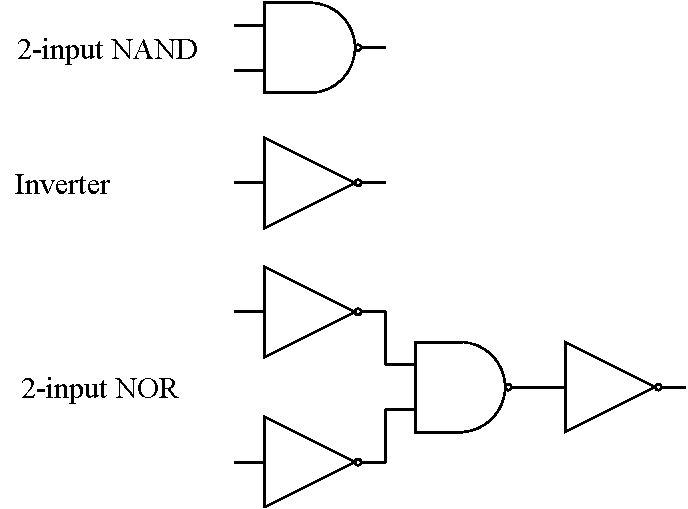
\includegraphics[width=0.5\linewidth]{3_1.pdf}
    \caption{Library patterns for the gates in the library.}
    \label{fig:library_patterns}
\end{figure}

{\color{statement} Consider the following function:
\[f = a_1b_1+a_2b_2+a_3b_3+a_4b_4\]
Draw the most balanced target graph in terms of the base functions and find the most efficient mapping.}

I started drawing the tree of the boolean operations of $f$ (see figure~\ref{fig:tree_f}). Using the library patterns, I created simple versions of AND ($\land$) and OR ($\lor$) gates. AND is formed by NAND and an inverter, and OR by NOR and an inverter. With the tree and these new gates, I drew the initial circuit, which is shown in figure~\ref{fig:init_circuit}. Blue indicates an area cost of 2 and green of 1. Hence, the initial circuit has an area cost of $2\times7 + 7 = 21$. 
\begin{figure}[htbp]
    \centering
    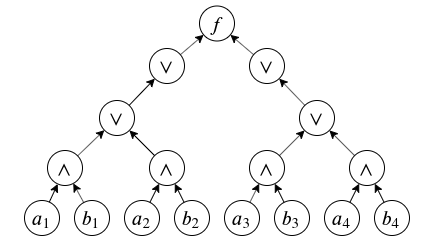
\includegraphics[width=0.5\linewidth]{3_2_1.png}
    \caption{Tree of $f$.}
    \label{fig:tree_f}
\end{figure}


\begin{figure}[htbp]
    \centering
    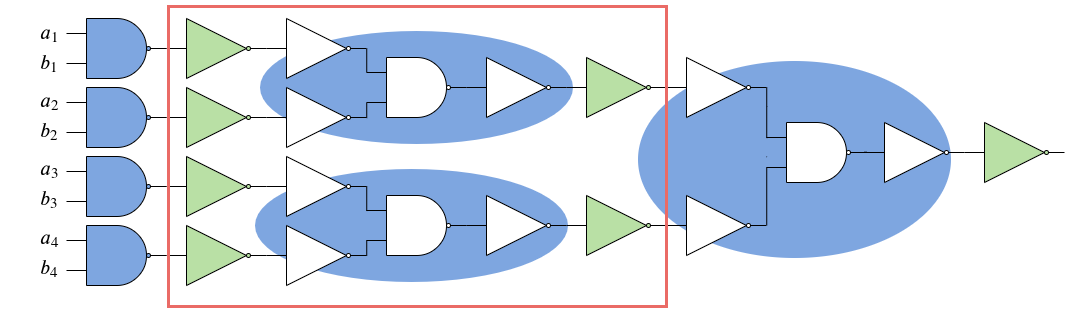
\includegraphics[width=\linewidth]{3_2_2.png}
    \caption{Initial circuit.}
    \label{fig:init_circuit}
\end{figure}

It is easy to see that the part of the initial circuit within the red rectangle (red zone) can be changed by two NAND gates, removing all two consecutive inverters in the zone. The area cost of the red zone goes from 10 to 4. The resultant circuit is shown in figure~\ref{fig:best_mapping}, and have an area cost of $7\times2 + 1 = 15$.

\begin{figure}[htbp]
    \centering
    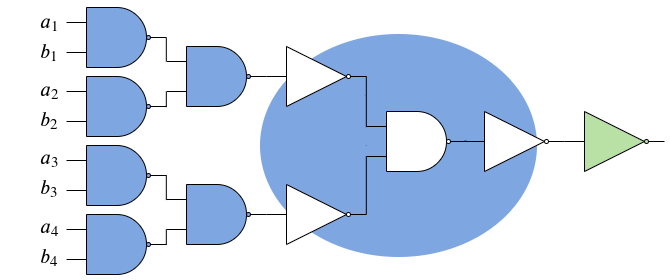
\includegraphics[width=0.7\linewidth]{3_2_3.png}
    \caption{Most efficient mapping.}
    \label{fig:best_mapping}
\end{figure}

Now, the only optimization you can do is to remove the two consecutive inverters at the end of the circuit, with leads to the one in figure~\ref{fig:last_circuit}. Unless this is the circuit with less gates, it has an area cost of $7\times2 + 2 = 16$, because removing the inverters it loses the NOR gate, increasing the cost by 1. So, the most efficient mapping is the one in figure~\ref{fig:best_mapping}.

\begin{figure}[htbp]
    \centering
    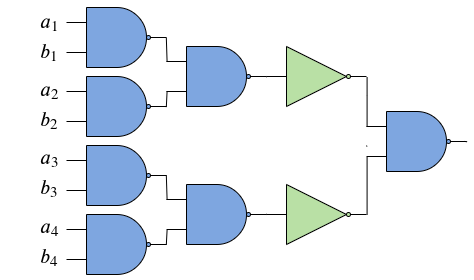
\includegraphics[width=0.5\linewidth]{3_2_4.png}
    \caption{Circuit with less gates.}
    \label{fig:last_circuit}
\end{figure}

{\color{statement} Let us assume that every gate has delay $=1$ and that the arrival time of all signals is $t = 0$, except for $b_4$ whose arrival time is $t = 10$. Draw the target graph that minimizes delay and find the most efficient mapping.}

I started drawing the tree of the boolean operations of $f$ (see figure~\ref{fig:tree_f_delay}). I build it taking into account that the arrival time of $b_4$ is 10. Then, I applied the same method that in previous question. You can see the resultant circuit in figure~\ref{fig:init_circuit_delay}. After that, I removed the two consecutive inverters within the red zone. Only one of them is maintained because it will not affect to the final delay (as I show later) and with this one NOR gate is maintained. With this, I obtained the most efficient mapping (area cost of 15, as in the previous question) with the minimum possible delay, which is 12.

\begin{figure}[htbp]
    \centering
    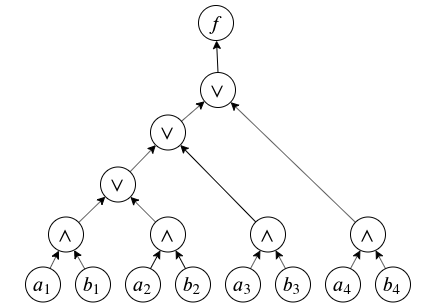
\includegraphics[width=0.5\linewidth]{3_3_1.png}
    \caption{Tree of $f$ with the critical delay path at $b_4$.}
    \label{fig:tree_f_delay}
\end{figure}


\begin{figure}[htbp]
    \centering
    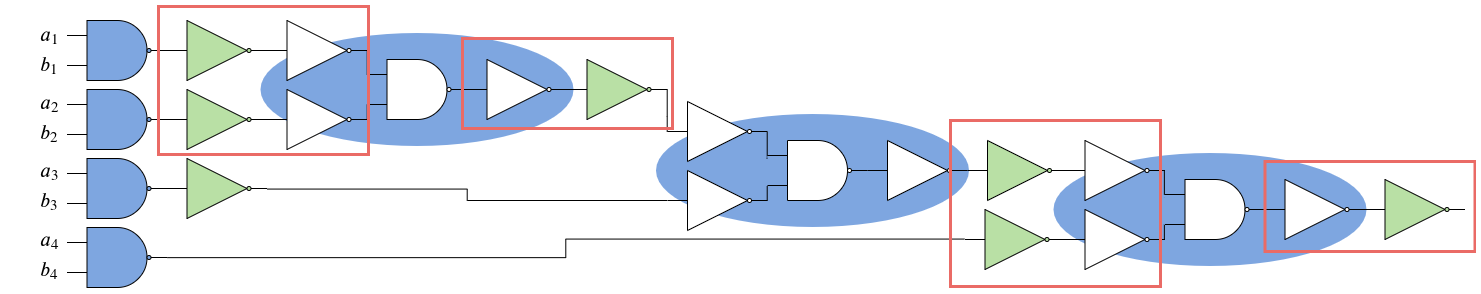
\includegraphics[width=\linewidth]{3_3_2.png}
    \caption{Initial circuit.}
    \label{fig:init_circuit_delay}
\end{figure}


\begin{figure}[htbp]
    \centering
    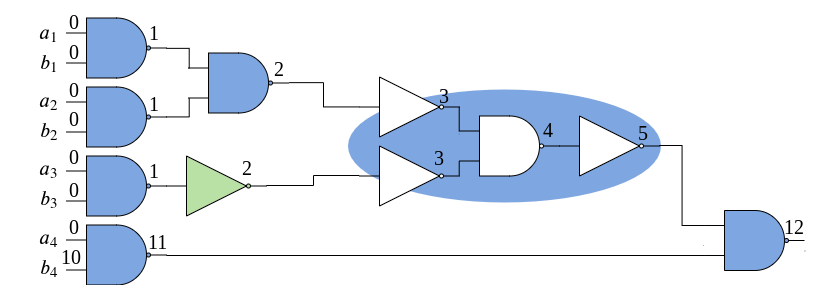
\includegraphics[width=0.7\linewidth]{3_3_3.png}
    \caption{Most efficient mapping with less delay.}
    \label{fig:best_mapping_delay}
\end{figure}

\section{Binary Decision Diagrams}
{\color{statement} Let us consider two Boolean vectors, $(a_{n-1}, ..., a_0)$ and $(b_{n-1} , ..., b_0)$, representing the binary encoding of two natural numbers $a$ and $b$. Let us consider the BDD of a Boolean function that is true when $a < b$ and false when $a \geq b$.

Justify the following answers and give an asymptotic complexity (using $O()$) of the BDD size for each case. Draw the BDD of the function considering the best variable order.} 

{\color{statement} What is the variable order that minimizes the BDD size?}

If the BDD starts from bit $n-1$, for each bit $i$ the BDD only has to check whether $a_{i} < b_{i}$ to return \textit{true}, $a_{i} > b_{i}$ to return \textit{false}, or $a_{i} = b_{i}$ to continue. This leads to a BDD like the one in figure~\ref{fig:min_bdd} (first BDD). It has $n$ nodes for $a$ and $2n$ nodes for $b$.Then, the size of this BDD is $3n$ ($O(n)$). The BDD of the figure~\ref{fig:min_bdd} starts with $a_{n-1}$ but can be done starting with $b_{n-1}$ in the same way.

\begin{figure}[htbp]
    \centering
    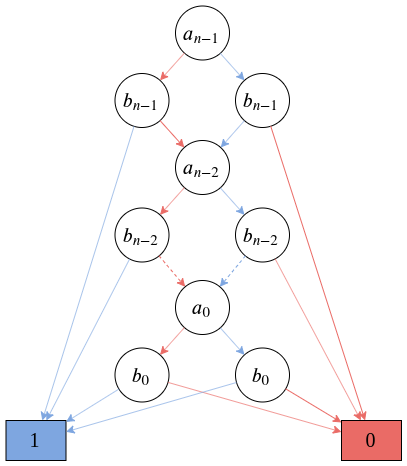
\includegraphics[width=0.35\linewidth]{min_bdd.png}
    \caption{BDD of the function with the order that minimizes the size.}
    \label{fig:min_bdd}
\end{figure}

{\color{statement} What is the variable order the maximizes the BDD size?}

If the BDD starts from bit $0$ with variable $a$, and considering $a_j$ (with $0 < j < n$) as a saving state (saving whether $(a_{0},...,a_{j}) > (b_{0},...,b_{j})$ or $(a_{0},...,a_{j}) \geq (b_{0},...,b_{j})$), the BDD in figure~\ref{fig:max_bdd} (second BDD) is obtained. It can be also done starting with $b$ and using $b_j$ as a saving state. The size of this BDD is $2+4(n-1)$ ($O(n)$).
\begin{figure}[htbp]
    \centering
    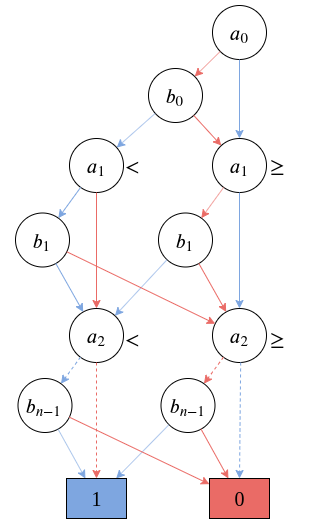
\includegraphics[width=0.3\linewidth]{max_bdd.png}
    \caption{BDD of the function with the order that maximizes the size.}
    \label{fig:max_bdd}
\end{figure}

Although the asymptotic complexity of the first BDD is the same than the other, their sizes are not ($3n < 2+4(n-1)$ for $n>1$). Furthermore, the first BDD can stop when checking each bit, only in the worst case (when $a = b$) it goes through all the BDD. The second BDD always does the latter.

\end{document}